\chapter{Desarrollo Experimental}   %\label{chap_content}
\minitoc

\section{Metodolog\'ia: Descripci\'on de caracterizaci\'on \'optica}


\begin{description}
\item[Fabricaci\'on de nanopart\'iculas.]  Un conjunto de materiales org\'anicos, que de acuerdo a su dise\~{n}o, podr\'ian presentar propiedades \'opticas de inter\'es para desarrollar marcadores biocompatibles, se utilizaron para fabricar suspensiones acuosas de nanopart\'iculas mediante el m\'etodo de reprecipitaci\'on. Se utilizaron principalmente semiconductores org\'anicos y mol\'eculas de tama\~{n}os variables.

\item[Caracterizaci\'on lineal.] Esta caracterizaci\'on \'optica de los materiales se realiz\'o en soluciones y en suspensiones acuosas de nanopart\'iculas; se adquirieron espectros de absorci\'on con un espectrofot\'ometro y espectros de emisi\'on lineal utilizando como excitaci\'on un diodo l\'aser de 370$nm$. Se midi\'o la eficiencia cu\'antica de fluorescencia utilizando el m\'etodo de la esfera integradora. 

\item[Caracterizaci\'on no lineal.] Se determin\'o la secci\'on transversal de absorci\'on de dos fotones $\sigma^{TPA}$ para soluciones y suspensiones de nanopart\'iculas del material precursor, utilizando la t\'ecnica de emisi\'on inducida por absorci\'on de dos fotones: se adquirieron espectros de emisi\'on no lineal utilizando l\'aseres de pulsos de femtosegundos en el rango espectral de inter\'es biom\'edico (730- 840$nm$ y/o 600- 900$nm$).

\item[Funcionalizaci\'on.] Las nanopart\'iculas que presentaron los valores m\'as grandes de eficiencia cu\'antica de fluorescencia y de secci\'on transversal de absorci\'on de dos fotones se funcionalizaron utilizando polietilenglicol PEG. Este PEG (con m\'ultiples grupos funcionales) se utiliz\'o como agente surfactante y estabilizador y para recubrir y modificar la superficie de las nanopart\'iculas de los materiales precursores. 

\item[Fotoestabilidad.]  Se estudi\'o la fotoestabilidad degradando las nanopart\'iculas funcionalizadas en celdas de cuarzo de 1$mm$ con una l\'ampara de xen\'on de 150$W$ y monitoreando los espectros de absorci\'on a diferentes tiempos.

\item[Tinci\'on de c\'elulas con nanoparticulas.] Las suspensiones acuosas de nanopart\'iculas funcionalizadas con PEG se internalizaron en l\'ineas celulares epiteliales y se obtuvieron im\'agenes de su distribuci\'on en la c\'elula con un microscopio de epifluorescencia. 

\end{description}

\section{Materiales y reactivos}\label{matis}

Se estudi\'o un grupo de 15 mol\'eculas fluorescentes sintetizados por la M.C. Mariana Flores y el Dr. Alejandro Alvarez Hern\'andez del Centro de Investigaciones en Qu\'imica, de la Universidad Aut\'onoma del Estado de Hidalgo; \'estas se basan en una mol\'ecula poliinsaturada con un grupo funcional amida y dos sustituyentes $R$. La estructura molecular y los 15 diferentes sustituyentes se muestran en la figura \ref{muchacha}.

Se trabaj\'o tambi\'en con un copol\'imero de dos bloques conocido como PF2/6-b-P3TMAHT, compuesto por el politiofeno
poli(9,9-dialquilfluoreno)-b-poli[3-(6-amoniohexil)tiofeno] (P3TMAHT) y el homopolifluoreno 2-(etil)hexil (PF2/6). Este copol\'imero, mostrado en la figura \ref{copolimerito}, fue proporcionado por el Dr. Ullrich Scherf de Bergische Universit\"at Wuppertal, Macromolecular Chemistry Group and Institute for Polymer Technology.

\begin{figure}[H]
\centering
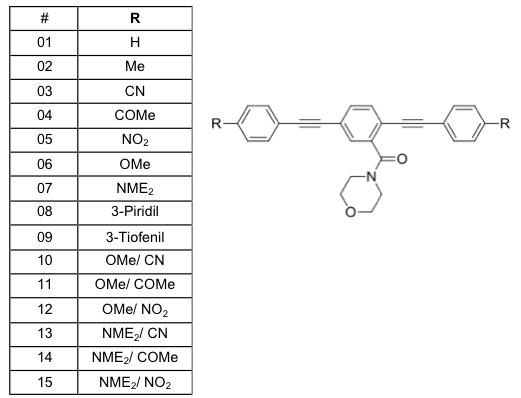
\includegraphics[width=0.85\textwidth]{desarrollo_experimental/HIDALGO}
\caption{15 sustituyentes $R$ en la estructura principal de la mol\'ecula \label{muchacha}}
\end{figure}


\begin{figure}[H]
\centering
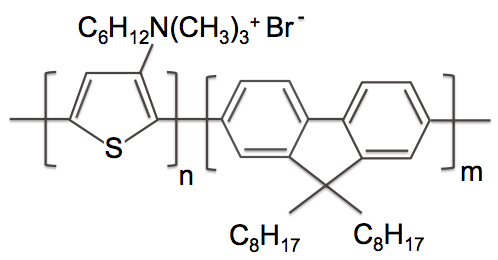
\includegraphics[width=0.55\textwidth]{desarrollo_experimental/copolimero}
\caption{Copol\'imero de dos bloques\label{copolimerito}}
\end{figure}



Por otra parte se estudiaron tres sistemas $\pi$ conjugados con diferente distribuci\'on de carga: etinilfluoreno-nitrilo (sistema dipolar) al que se har� referencia como 1NDS, etinilfluoreno-piridazina (sistema cuadrupolar) � 2NQS y etinilfluoreno-triazina (sistema octopolar) � 3NOS; en la figura \ref{ar2} se muestran las estructuras de estos sistemas basados en unidades de fluoreno. Los pesos moleculares $M_{w}$ son $515.771g/mol$, $905.387 g/mol$ y $1547.312g/mol$ para la mol\'ecula dipolar, cuadrupolar y octopolar respectivamente. Las mol\'eculas fueron dise\~{n}adas y sintetizadas por el Dr. Arturo Jim\'enez y la Dra. Rosa Santill\'an del Departamento de Qu\'imica Cinvestav- IPN.

\begin{figure}[h]
\centering
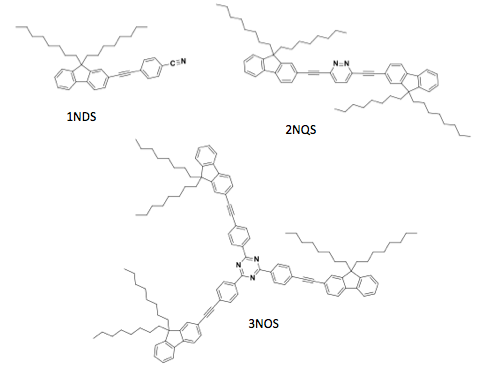
\includegraphics[width=\textwidth]{desarrollo_experimental/arturo}
\caption{Mol\'eculas org\'anicas dipolar, cuadrupolar y octopolar\label{ar2}}
\end{figure}

Finalmente se estudio tambi\'en el pol\'imero derivado de fluoreno PMC300 (Ver Figura \ref{PMC}), el cual est\'a basado en el mon\'omero 4,7-bis[2-(9,9-dimetil)fluorenil]benzo[1,2,5]tiadiazol; la s\'intesis se ha reportado por G. Ramos-Ort�z et al. \cite{laura}.

\begin{figure}[H]
\centering
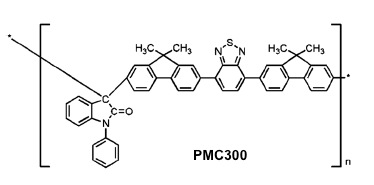
\includegraphics[width=0.7\textwidth]{desarrollo_experimental/PMC300}
\caption{Pol\'imero PMC300\label{PMC}}
\end{figure}

En este trabajo se utiliz\'o el colorante comercial Rodamina 6G de Sigma-Aldrich, principalmente como referencia. La Rodamina 6G es una mol\'ecula fluorescente cuyas propiedades \'opticas lineales y no lineales han sido ampliamente estudiadas, tiene una eficiencia cu\'antica de fluorescencia de 0.95 y presenta una alta fotoestabilidad, adem\'as es un material que puede conseguirse f\'acilmente a un costo relativamente bajo.

\begin{figure}[H]
\centering
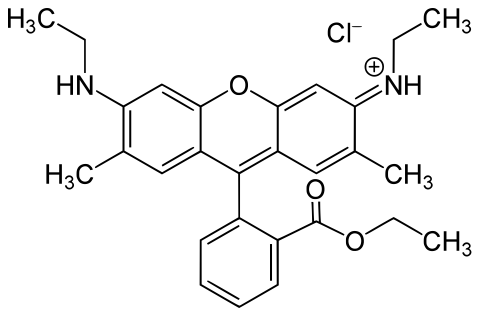
\includegraphics[width=0.55\textwidth]{desarrollo_experimental/rodamina6g}
\caption{Rodamina 6G\label{laroda}}
\end{figure}

Para recubrir las nanopart\'iculas se utilizaron dos tipos de polietilenglicol, PEG 5000 adquirido de Sigma-Aldrich y PEG 2000 de Avanti Polar Lipids Inc., el peso molecular promedio $M_n$ es de $5000g/mol$ y $2000g/mol$ respectivamente. Sus estructuras qu\'imicas se muestran en la figura \ref{pegs}.

\begin{figure}[H]
\centering
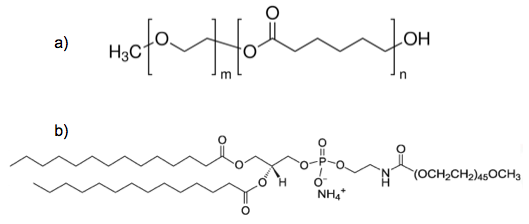
\includegraphics[width=0.85\textwidth]{desarrollo_experimental/peg}
\caption{Estructuras de a) PEG 5000 y b) PEG 2000 \label{pegs}}
\end{figure}


%poner que es thf, ctab y todos los nombres completos de los reactivos 

%peg 2000 y peg 5000


\section{Fabricaci\'on de nanopart\'iculas por el m\'etodo de reprecipitaci\'on}

El m\'etodo de reprecipitaci\'on se basa en la diferencia de solubilidad que tiene el material precursor en una mezcla compuesta por un buen disolvente y un mal disolvente para dicho precursor, ambos miscibles \cite{reprecipita}. La creaci\'on de este sistema mediante una mezcla r\'apida provoca una precipitaci\'on local y la nucleaci\'on de nanopart\'iculas en lugar de una precipitaci\'on en bulto \cite{coloidal}.

El proceso de reprecipitaci\'on para la fabricaci\'on de suspensiones acuosas de nanopart\'iculas de los sistemas org\'anicos a estudiar (Ver Figura \ref{fig_repreci}), es el siguiente:

\begin{description}
\item[$\circ$]  Preparaci\'on de una soluci\'on madre en THF a una concentraci\'on de $1\times10^{-3}$ \'o $1\times10^{-4} M$ dependiendo del peso molecular del material precursor.
\item[$\circ$]  Se realiz\'o una soluci\'on de un surfactante en agua a una concentraci\'on de 0.8 $mM$. El surfactante m\'as utilizado fue el CTAB aunque tambi\'en se realizaron pruebas con Trit\'on- X 100  
\item[$\circ$]  Utilizando jeringas de insulina se inyectaron r\'apidamente 0.5$ml$ de la soluci\'on madre en 8$ml$ de la soluci\'on acuosa bajo sonicaci\'on para causar la nucleaci\'on de nanopart\'iculas a una concentraci\'on de $1\times10^{-5}$ a $1\times10^{-7} M$ dependiendo del material.
\item[$\circ$]  Como se busc\'o desarrollar marcadores biocompatibles, se evapor\'o el disolvente t\'oxico de la suspensi\'on acuosa de nanopart\'iculas\footnote{De acuerdo con la literatura, �ste tipo de m�todo de fabricaci�n de nanopart�culas puede desarrollar marcadores o portadores de f�rmacos biocompatibles al evaporar el disolvente, ya que el surfactante recubre las nanopart�culas del material precursor y cambia la solubilidad de �ste �ltimo, en agua. Ver por ejemplo referencia \cite{artconcluyente}.}. La suspensi\'on se introdujo en un matraz de Kitasato haciendo vac\'io con una bomba de extracci\'on.
\end{description}

\begin{figure}[H]
\centering
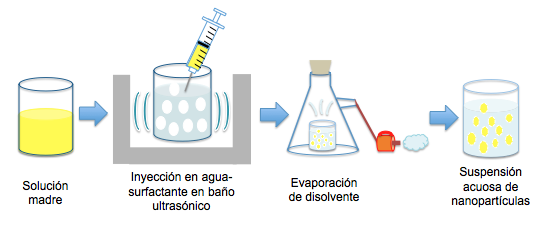
\includegraphics[width=1\textwidth]{desarrollo_experimental/reprecipitacion}
\caption{M\'etodo de reprecipitaci\'on}\label{fig_repreci}
\end{figure}

El surfactante act\'ua como un agente estabilizador en la suspensi\'on acuosa de nanopart\'iculas. El tama\~{n}o de \'estas se puede controlar  modificando la concentraci\'on de la soluci\'on madre y el disolvente.

\subsection{Recubrimiento de nanopart\'iculas con PEG}\label{pegis}

Los dos tipos de PEG que se utilizaron en este trabajo son anfif�licos y tienen los grupos funcionales: \'eter, \'ester y alcohol en el caso del PEG 5000 y \'ester, varios grupos \'eter, fosfato, amonio y amida en el PEG 2000 (Grupos funcionales mencionados de izquierda a derecha en las estructuras de la figura \ref{pegs}). As�, al utilizarlos para recubrir las nanopart\'iculas, se modific� la superficie de las mismas y se llev� a cabo una funcionalizaci\'on.

Para realizar la funcionalizaci�n de nanopart�culas se utiliz� el m�todo de reprecipitaci�n (Ver Figura \ref{fig_repreci}), reemplazando al surfactante por PEG. Con el PEG 5000 se prepar\'o una soluci\'on acuosa a una concentraci\'on de $4\times10^{-6} M$, debido a que \'este se precipitaba en soluciones acuosas a concentraciones mayores o iguales a $1\times10^{-5} M$. Y nuevamente a 8$ml$ de \'esta soluci\'on se inyectaron 0.5$ml$ de la soluci\'on madre del material precursor de inter\'es, para formar una suspensi\'on acuosa de nanopart\'iculas funcionalizadas con este PEG a concentraciones del orden de $10^{-6} M$. Posteriormente el disolvente fue evaporado.

El PEG 2000 present\'o m\'as estabilidad, para este caso la soluci\'on acuosa pudo prepararse a una concentraci\'on de $6\times10^{-4} M$ (Concentraci\'on del orden de magnitud m\'as reportado en la literatura). Las suspensiones acuosas de nanopart\'iculas tuvieron concentraciones entre $10^{-6}$ y $10^{-7} M$, inyectando 0.5$ml$ de la soluci\'on madre en 8$ml$ de la soluci\'on acuosa y despu\'es de evaporar el disolvente.

%\subsubsection{Transferencia de energ\'ia de resonancia F\"orster}

%\subsubsection{PEG 5000}
%Con este PEG se funcionalizaron las nanopart\'iculas de la mol\'ecula octopolar 3NOS. Inicialmente se prepar\'o la soluci\'on madre a una concentraci\'on de $1\times10^{-4} M$ y se realiz\'o una soluci\'on acuosa de PEG 5000 a una conc�ntrica\'on de $4\times10^{-6} M$. Se inyectaron 0.5$ml$ de soluci\'on madre en 8$ml$ de la soluci\'on acuosa para obtener una suspensi\'on acuosa de nanopart\'iculas a una concentraci\'on de $6.4\times10^{-6} M$ y posteriormente se evapor\'o el disolvente.

%\subsubsection{PEG 2000}
%Las nanopart\'iculas del pol\'imero PMC300, PMC300 dopado con Rodamina 6G, de la mol\'ecula octopolar y del dendr\'imero se funcionalizaron con PEG 2000. Se prepararon las soluciones madre del pol\'imero PMC300 a una concentraci\'on de $5.9\times10^{-6} M$; una soluci\'on de este pol\'imero (misma concentraci\'on) dopada con Rodamina 6G al 177, 100 y 50\% molar; la soluci\'on de la mol\'ecula octopolar a $1\times10^{-4} M$  y del dendr\'imero a una concentraci\'on de $1.1\times10^{-4} M$.

%En este caso, la soluci\'on acuosa de PEG 2000 se prepar\'o a una concentraci\'on de $1\times10^{-4} M$. 

%Se inyectaron 0.5$ml$ de las soluciones madre en 8$ml$ de las soluciones acuosas para cada compuesto; obteniendo  suspensiones acuosas con concentraciones de $3.5\times10^{-7} M$,$3.5\times10^{-7} M$ de PMC300/ $1.75\times10^{-7} M$ de Rodamina 6G, de $6.4\times10^{-6} M$ y de $6.9\times10^{-6} M$ para las nanopart\'iculas de PMC300, PMC300 con Rodamina 6G al 50\% molar, de la mol\'ecula octopolar y el dendr\'imero respectivamente. Posteriormente se evapor\'o el disolvente.
\section{Espectros de absorci\'on y emisi\'on lineal}

Los espectros de absorci\'on de las soluciones y suspensiones acuosas de nanopart\'iculas se obtuvieron con el espectrofot\'ometro  Perkin Elmer modelo Lambda 900 en un rango de 250 a 900$nm$. Las soluciones y suspensiones se colocaron en celdas de cuarzo de $0.1\times1\times4 cm^{3}$ \'o $1\times1\times4 cm^{3}$ dependiendo de la concentraci\'on y la absorbancia de cada muestra.

Los espectros de emisi\'on lineal se obtuvieron con un espectr\'ometro port\'atil Ocean Optics USB4000, excitando las muestras con un diodo l\'aser emitiendo a 370$nm$ como se muestra en la figura \ref{emilineal}. El haz de excitaci\'on enfocado con la lente L1 incide en la muestra contenida en la celda, la luz emitida es recolectada con un sistema de lentes perpendicular al haz de excitaci\'on; la lente L2 colecta la fluorescencia y la colima; la lente L3 forma la imagen del volumen excitado en la abertura del espectrometro. El espectrometro est\'a sobre una montura XY que permite su alineaci\'on para detectar mayor fluorescencia y utilizando el programa Spectra Suite, se pueden visualizar y guardar los espectros de emisi\'on.

\begin{figure}[h]
\centering
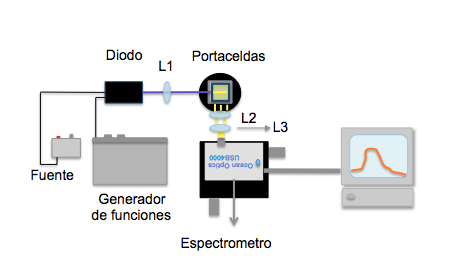
\includegraphics[width=0.9\textwidth]{desarrollo_experimental/emision_lineal}
\caption{Arreglo experimental para medir emisi\'on lineal}\label{emilineal}
\end{figure}

Es necesario guardar un espectro de emisi\'on con el diodo l\'aser apagado para detectar la se\~{n}al de fondo y restarla de los espectros de emisi\'on obtenidos para cada muestra. 

El diodo l\'aser se modul\'o con un generador de funciones: amplitud de 0 $Vpp$ y un Offset de 1V. Para evitar la saturaci\'on del espectrometro se utilizaron filtros neutros de densidad \'optica variable entre la fuente de excitaci\'on y la muestra o bien, se redujo el valor del offset. 

\section{Medici\'on de eficiencia cu\'antica de fluorescencia}

La eficiencia cu\'antica de fluorescencia de los materiales estudiados se midi\'o en soluciones y/o suspensiones de nanopart\'iculas, colocando \'estas en una celda de cuarzo de $0.1\times1\times4 cm^{3}$. En el arreglo experimental se utiliz\'o un diodo l\'aser a 370$nm$ como fuente de excitaci\'on, un diafragma $D1$, dos lentes $L1$ y $L2$, una esfera integradora de 25.4$cm$ de di\'ametro interno, modelo INS250 de International Light Technologies; un tubo fotomultiplicador o PMT por sus siglas en ingles (serie R7400U de Hamamatsu) colocado a 90$^{\circ}$ del haz de excitaci\'on y un amplificador lock- in modelo SR830 de Stanford Research Systems, como se muestra en la figura \ref{eficiencia}. 

\begin{figure}[h]
\centering
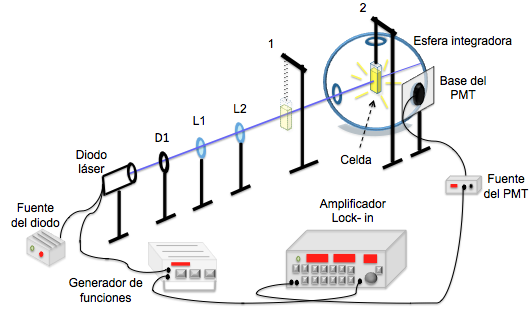
\includegraphics[width=1\textwidth]{desarrollo_experimental/arreglo_qy}
\caption{Arreglo experimental para obtener la eficiencia cu\'antica de fluorescencia}\label{eficiencia}
\end{figure}

El diodo l\'aser de 370$nm$ se modul\'o con el generador de funciones utilizando regularmente una se\~{n}al cuadrada con frecuencia de 60$Hz$, amplitud de 1$Vpp$ y offset de 0.5$V$; \'esta se\~{n}al se utiliz\'o como referencia en el amplificador lock- in. Con el diafragma $D1$ se realiz\'o un filtrado espacial de la luz, la lente $L1$ enfoc\'o el haz y la lente $L2$ se utiliz\'o para colimar la luz. La celda se coloc\'o en bases fijas fuera y dentro de la esfera (Ver Figura \ref{eficiencia}) en las posiciones 1 y 2 respectivamente. 

En la esfera, a pesar de los filtros, la luz reflejada internamente proviene del haz de excitaci\'on residual, fluorescencia de la muestra y ruido; y es detectada por el PMT\footnote{El PMT se encendi\'o utilizando 200 V en todas las mediciones}. Sin embargo, en el amplificador lock- in se utiliz\'o la frecuencia del generador de funciones como referencia para discriminar el ruido y luz proveniente de otras fuentes. Los valores entregados por el lock- in se dieron en volts $V$.

Se utiliz\'o Rodamina 6G (Ver Figura \ref{laroda}) como colorante de referencia para calcular las eficiencias cu\'anticas de los compuestos de inter\'es. La celda se coloc\'o en las posiciones 1 y 2 mostradas en la figura \ref{eficiencia} para detectar solamente la fluorescencia: en la posici\'on 2, la luz de excitaci\'on transmitida por la celda, fluorescencia del compuesto y ruido se detectaron; mientras que en la posici\'on 1 solo la luz de excitaci\'on transmitida y el ruido. Entonces para cada muestra (incluida la referencia) se rest\'o el valor arrojado por el amplificador en la posici\'on 1 al valor obtenido en la posici\'on 2 y obtener idealmente  luz emitida por el compuesto en soluci\'on o suspensi\'on.

La superficie de mayor \'area en la celda se aline\'o perpendicular a la direcci\'on de propagaci\'on de la luz de excitaci\'on para evitar que el haz reflejado se quedara en el interior de la esfera integradora.
 
Debido a la sensibilidad del PMT, este s\'olo se encend\'ia hasta que la celda era colocada en las posiciones preestablecidas y despu\'es de ser alineadas con el haz de excitaci\'on. Para evitar da\~{n}ar este fotomultiplicador solo se dejaba encendido el instante en el que se registraban los valores arrojados por el amplificador. Se intentaba aislar de cualquier tipo de luz externa el sitio en el que se mont\'o el arreglo experimental mientras el PMT se encontraba encendido. Adem\'as la pantalla dentro de la esfera, entre la muestra y el sistema de detecci\'on, se utiliz\'o para proteger el PMT de la detecci\'on directa de la luz de excitaci\'on y/o fluorescencia; tambi\'en se colocaron filtros UV entre la salida de la esfera y el PMT, para atenuar la luz de excitaci\'on.

Las soluciones y suspensiones acuosas de nanopart\'iculas con las que se trabaj\'o, ten\'ian concentraciones bajas de $1\times10^{-5}$ a $1\times10^{-7} M$ para evitar interacciones y procesos, que por la proximidad de las  mol\'eculas, pudieran  llevar a la disminuci\'on de fluorescencia. En las muestras que aun a bajas concentraciones presentaban una gran emisi\'on de luz se utilizaron filtros neutros de densidad \'optica variable o se modificaban los par\'ametros del generador de funciones (para as\'i disminuir el nivel de excitaci\'on).

\section{Medici\'on de $\sigma^{TPA}$ de 740 a 840 nm}\label{laserlau}

La secci\'on transversal de absorci\'on de dos fotones de las suspensiones acuosas de nanopart\'iculas y soluciones del material de inter\'es se midieron mediante la t\'ecnica de TPEF, adquiriendo los espectros de emisi\'on inducida por absorci\'on de dos fotones. Para ello se utiliz\'o un l\'aser de Titanio: Zafiro con pulsos de 100 $fs$ de duraci\'on y frecuencia de repetici\'on de 80 $MHz$ en un rango de 725-- 860 $nm$ (modelo \emph{Tsunami}-3955 de Spectra-Physics); este l\'aser fue bombeado por un l\'aser de onda continua \emph{Millennia Pro s- Series} a 532 $nm$ con una potencia de 5 Watts.

En la figura \ref{sencillotpa} se aprecia el arreglo experimental; a la salida del l\'aser de Ti:Za se coloc\'o un retardador de media longitud de onda y un aislador de Faraday (componente $A$) para controlar la intensidad de excitaci\'on, se desvi\'o el haz utilizando cuatro espejos $M1$-$M4$ para no interferir con otros arreglos colocados sobre la mesa \'optica de trabajo, el diafragma $D1$ se utiliz\'o como referencia para alinear los componentes \'opticos, la lente $L1$ enfoc\'o el haz en una celda de cuarzo de $1\times1\times4 cm^3$ con la soluci\'on o suspensi\'on de inter\'es y con el sistema de lentes $L2$ y $L3$, colocadas de manera perpendicular al haz incidente, se colect\'o y dirigi\'o la fluorescencia inducida por absorci\'on de dos fotones a la abertura del espectr\'ometro port\'atil Ocean Optics USB4000. 

Idealmente la lente $L2$ colima la luz mientras que la lente $L3$ la enfoca en la abertura del espectrometro, \'este se encontraba sobre una montura XY para detectar la mayor cantidad de fluorescencia, y para visualizar y guardar los espectros de emisi\'on se utiiz\'o el programa Spectra Suite. El haz de excitaci\'on se enfoc\'o en un extremo de la celda de cuarzo, muy cercano a una de sus paredes para reducir la distancia entre el volumen excitado y las lentes colectoras de luz, disminuyendo as\'i la atenuaci\'on de fluorescencia debida a efectos de absorci\'on.

\begin{figure}[h]
\centering
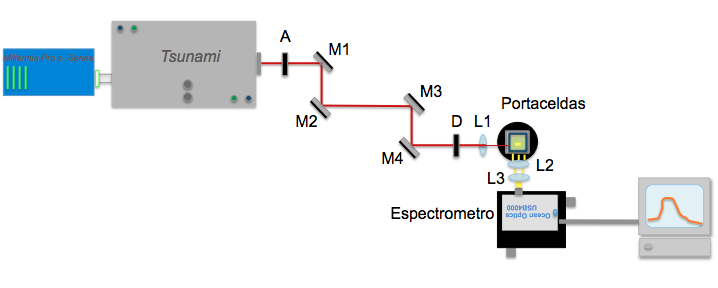
\includegraphics[width=1\textwidth]{desarrollo_experimental/tpa}
\caption{Arreglo experimental para medir $\sigma^{TPA}$ (Rango 740-- 840 $nm$)}\label{sencillotpa}
\end{figure}

Como muestra de referencia se utiliz\'o  Rodamina 6G a una concentraci\'on de $1\times 10^{-4} M$. Los espectros de emisi\'on no lineal de las nanopart\'iculas o soluciones y de la referencia, fueron obtenidos bajo las mismas condiciones con una potencia incidente de 410 $mW$ \footnote{Esta potencia se midi\'o a la salida del aislador de Faraday} y para 11 diferentes longitudes de onda de excitaci\'on: de 740 a 840 $nm$ cada 10 $nm$. Adem\'as, para cada longitud de onda se guard\'o la se\~{n}al detectada por el espectrometro al bloquear el haz de excitaci\'on para restar esta se\~{n}al de fondo a los espectros de cada muestra incluida la referencia. 

El l\'aser de Ti:Za se sintoniz\'o girando dos tornillos de movimiento microm\'etrico ubicados en la parte superior del l\'aser. Uno de ellos cambia la posici\'on de una rendija que modifica la longitud de onda y el otro tornillo mueve un compensador de dispersi\'on, formado por cuatro prismas.

\section{Medici\'on de $\sigma^{TPA}$ de 650 a 760 nm}\label{laserchidote}

Para medir $\sigma^{TPA}$ en este rango mediante la t\'ecnica TPEF se utiliz\'o un amplificador ultrarr\'apido (basado en un l\'aser de Ti:Za) modelo Libra- HE de Coherent, con emisi\'on de pulsos de 50 $fs$ de duraci\'on, frecuencia de repetici\'on de 1 $kHz$ y longitud de onda central de 800nm; adicionalmente se utiliz\'o un amplificador \'optico param\'etrico modelo TOPAS- C de Light Conversion capaz de sintonizar la longitud de onda en un rango continuo de 290 a 2600 $nm$. Como sistema de detecci\'on se utiliz\'o un monocromador/espectr\'ometro de la serie Acton SP-2500i de Princeton Instruments y un tubo fotomultiplicador o PMT por sus siglas en ingles de la serie R7400U de Hamamatsu.

\begin{figure}[h]
\centering
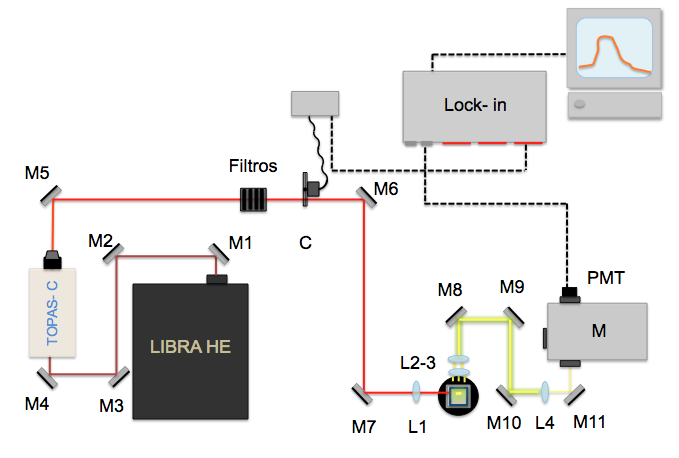
\includegraphics[width=1\textwidth]{desarrollo_experimental/tpa_femto}
\caption{Arreglo experimental para medir $\sigma^{TPA}$ (Rango 650-- 760 $nm$)}\label{mastpa}
\end{figure}

Como se aprecia en la figura \ref{mastpa} el amplificador \'optico param\'etrico TOPAS- C fue bombeado por el l\'aser Libra- HE utilizando los espejos $M1$-$M4$, el TOPAS- C se sintoniza y controla utilizando un programa computacional del equipo y a la salida de \'este, se coloca el filtro correspondiente para permitir la salida de la longitud de onda seleccionada. Utilizando el espejo $M5$, el haz de excitaci\'on se envi\'o a una serie de filtros de densidad \'optica variable para controlar la intensidad del haz y posteriormente el haz se modul\'o utilizando un chopper $C$ a una frecuencia de 39 $Hz$. Con los espejos $M6$ y $M7$ el haz se hizo incidir en la lente $L1$ para ser enfocado en una celda de cuarzo de $1\times1\times4 cm^3$; con las lentes $L2$- $L3$ se colect\'o la luz emitida por la muestra de inter\'es de manera perpendicular al haz incidente en la celda; utilizando los espejos $M8$-$M10$ la luz emitida se dirigi\'o a la lente $L4$ para enfocarla en la rendija de entrada del monocromador/ espectr\'ometro $M$ utilizando el espejo $M11$. 

A la salida del monocromador/ espectr\'ometro se coloc\'o un PMT, encendido con 900 $V$ en todas las mediciones, y se amplific\'o la se\~{n}al detectada con un amplifciador lock- in modelo SR830 de Stanford Research Systems, utilizando como referencia la se\~{n}al del chopper. Para poder visualizar y guardar los espectros de emisi\'on en base a los datos del amplificador lock- in, se utiliz\'o un software desarrollado por un miembro del GPOM\footnote{El software fue desarrollado por el Ing. f\'isico Manuel De Anda Villa para automatizar la detecci\'on y guardado de datos arrojados por el Lock-in de forma gr\'afica}. El haz de excitaci\'on se enfoc\'o muy cerca a una de las paredes de la celda de cuarzo para reducir la distancia entre el volumen excitado y las lentes colectoras de luz, disminuyendo as\'i la atenuaci\'on de fluorescencia.

Se utiiz\'o nuevamente Rodamina 6G como referencia a una concentraci\'on de $1\times 10^{-4} M$. Los espectros de emisi\'on no lineal de la muestra de referencia, suspensiones acuosas de nanopart\'iculas y soluciones fueron obtenidos bajo las mismas condiciones con una potencia incidente de entre 250 y 270 $\mu W$ para 12 diferentes longitudes de onda de excitaci\'on: de 650 a 760 $nm$ cada 10 $nm$. Y nuevamente para cada longitud de onda se guard\'o un espectro de la se\~{n}al detectada al bloquear el haz de excitaci\'on, para restar \'este fondo a los espectros de cada muestra de inter\'es incluida la referencia.

La medici\'on de $\sigma^{TPA}$ en este rango no se realiz\'o para todos los materiales estudiados, \'unicamente para los materiales de mayor inter\'es que presentaron los valores m\'as altos de $\sigma^{TPA}$ para el rango de 740 a 840 $nm$.

\section{Fotoestabilidad de las nanopart\'iculas}\label{fotitopalalupe}

Las soluciones y suspensiones acuosas de nanopart\'iculas de mayor inter\'es fueron sometidas a un estudio de fotoestabilidad; las muestras fueron expuestas a una l\'ampara UV durante 165 minutos, monitoreando los espectros de absorci\'on a diferentes tiempos. Las muestras se colocaron a 15 $cm$ de la l\'ampara para evitar que se calentaran demasiado y el disolvente se evaporara. 

El objetivo de este estudio fue comprobar que las soluciones sufren de un fotoblanqueado en un tiempo menor de exposici\'on a la luz comparadas con las suspensiones acuosas de nanopart\'iculas del mismo material.

\section{Internalizaci\'on de nanopart\'iculas en l\'ineas celulares epiteliales (L929)}\label{yacasicasi}

Las c\'elulas epiteliales L929 (Fibroblastos de rat\'on) son cultivadas\footnote{Se cont\'o con el apoyo de la Dra. Myrna Sabanero L\'opez del Laboratorio de Biolog\'ia Celular y Molecular de las Interacciones, de la Universidad de Guanjauato; la Dra. Sabanero proporcion\'o las l\'ineas celulares y desarroll\'o el protocolo y proceso de la tinci\'on celular.} en un medio DMEM (Dulbecco's Modified Eagle's Medium), el cual contiene amino\'acidos, sal, vitaminas, glucosa, hierro y rojo de fenol, suplementado con 10\% de suero fetal bovino y 0.1\% de antibi\'oticos y antimic\'oticos. Los cultivos se incubaron a una temperatura de 37$^{\circ} C$, con una atm\'osfera de 5\% de CO$_2$ y humedad constante.

Las nanopart\'iculas org\'anicas de mayor inter\'es por sus propiedades \'opticas, se internalizaron en las lineas celulares siguiendo el protocolo siguiente:

\begin{description}
\item[1.-]  Las c\'elulas se fijaron en cubreobjetos de 20$\times$20 $mm$ utilizando paraformaldehido 4\% y glutaraldehido 0.05\% en una soluci\'on salina de fosfato (PBS) durante 20 minutos.
\item[2.-]  Las c\'elulas fueron permeabilizadas utilizando Trit\'on 0.05\% durante tres minutos.
\item[3.-]  Se prepar\'o una sonda compuesta por suero fetal bovino y suspensi\'on acuosa de nanopart\'iculas en diferentes proporciones.
\item[4.-]  Las c\'elulas fueron expuestas a la sonda por un tiempo de 30 minutos.
\item[5.-]  El cubreobjetos con las c\'elulas y la sonda fue montado y sellado en un portaobjetos, adicionando DAPI (4 ',6-diamino-2-fenilindol) entre las laminillas. El DAPI es un marcador fluorescente que se une fuertemente al ADN o bien al n\'ucleo de las c\'elulas.
\item[6.-]  Finalmente el portaobjetos, con las nanopart\'iculas en las c\'elulas, se observ\'o con el microscopio de epifluorescencia modelo IX81 de Olympus.
\end{description}

Cabe mencionar que posterior al paso n\'umero 1, 2 y 4 las c\'elulas del cubreobjetos fueron lavadas suavemente utilizando PBS, ello para remover las c�lulas que no se fijaron, para retirar el surfactante no absorbido y limpiar las c�lulas de las nanopart�culas que no se internalizaron.




%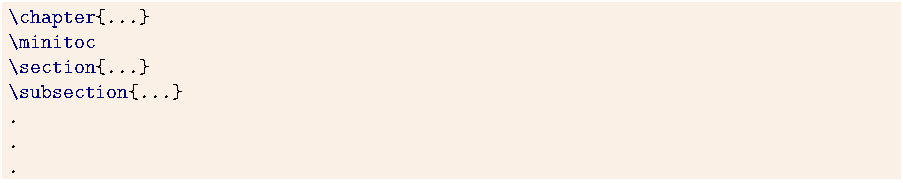
\includegraphics[width=\textwidth]{your_stuff/pre}

